\section{Smartphone Scan Rate}
\label{sec:scan}

\begin{figure}[t!]
  \centering
  \begin{subfigure}[t]{\columnwidth}
    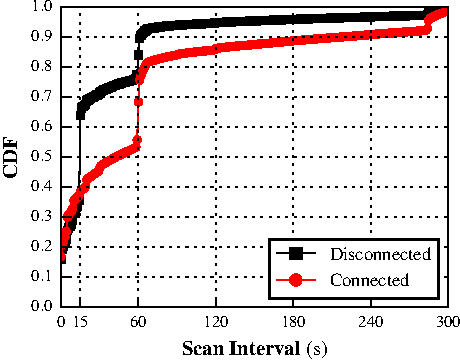
\includegraphics[width=\textwidth]{./figures/ScanIntervalGraph.pdf}
    \caption{\textbf{CDF of Android Natural Scan Intervals.}}
    \label{fig:android_interval}
  \end{subfigure}\\
  \begin{subfigure}[t]{\columnwidth}
    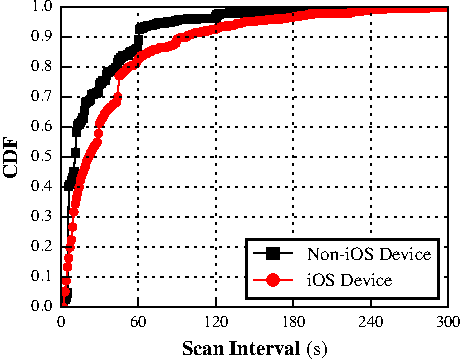
\includegraphics[width=\textwidth]{./figures/NDScanInterval.pdf}
    \caption{\textbf{CDF of iOS and non-iOS Devices Scan Intervals.}}
    \label{fig:ios_interval}
  \end{subfigure}
\caption{\textbf{Smartphone Natural Scan Rate.} Both Android and iOS systems perform
\wifi{} scans aggressively.}
  \label{fig:intervals}
  \vspace*{\aftercaptiongap}
\end{figure}

We first look at the natural \wifi{} scan rate of smartphones. The goal is to
evaluate the feasibility of passive wireless network monitoring using
smartphones without introducing extra scanning overhead. We focus on the two
most popular smartphone platforms, Android and iOS, which together occupy 96.3\%
of the market share as of Q4, 2014~\cite{smartphone-market-share}.

Android is configured to perform \wifi{} scans periodically to maintain an
up-to-date list of available APs. This is particularly important on smartphones
where mobility can cause network conditions to change rapidly. During a scan,
the phone sweeps each \wifi{} channel, sends out probe packets and waits for
probe responses from APs on that channel. When the scan completes, the phone
reports a list of scan results, the content of which is described in
Section~\ref{sec:phonelab}.

We studied the intervals between consecutive scans in \ubscan{} dataset. Since
the scan results were only passively collected whenever the Android system or
applications trigger scans, the intervals capture the devices' natural scanning
rate. Figure~\ref{fig:android_interval} shows the CDF of such scan intervals of
all devices in study, separated by whether the device is connected to an AP or
not. The periodic scan behavior can clearly be seen through the spikes in the
figure. In particular, when the phone is not connected to \wifi{}, Android
eagerly searches for potential APs by scanning every 15 seconds. Even when the
device is connected to \wifi{} networks, Android still scans at a relatively
lower frequency, every 60 seconds, to find potentially better APs.

We then use a second dataset~\cite{hu2015there} to understand the scan
behavior of iOS devices. The dataset was collected using laptops with Airpcap
packet sniffers deployed near gates of the football stadium at Notre Dame.  Data
was gathered over a ninety minute period prior to the start of the game and in
total, \num{82129} scans\footnote{A scan is identified by a burst of probe
packets from the same device.} from 2605 devices were captured, 1454 of which
were iOS devices. Figure~\ref{fig:ios_interval} shows the CDF of scan intervals
of both iOS and non-iOS devices. For non-iOS devices, we observe very similar
curves to the Android scan rate, probably because of them are actually Android
devices. For iOS devices, 80\% of the intervals are less than 1 minute, and
there are two spikes at 30 and 45 seconds, which probably correspond to the
periodic intervals adopted by iOS devices when device is disconnected and
connected to \wifi{} networks respectively.  

In summary, we confirmed that smartphones indeed naturally generate a stream of
network observations with high temporal granularity.
